\chapter{Feature selection}\label{ch:fs}

We introduce in this chapter the concepts of feature selection and false discovery rate control,
as well as a short review of a few methods that are usually employed.
Finally, we detail the knockoff framework developed by Barber-Candès,
a recent approach to control the false discovery rate when performing feature selection.

\section{Background on feature selection}\label{sec:bfs}

\subsection{Definitions}\label{subsec:fs_defs}

Feature selection is an active area of research in statistics and machine learning.
It primarily consists in identifying the most relevant features (or covariates) explaining an observed variable.
More formally, let $\cX$ be a $p$-dimensional random vector representing observed features
and $\cY$ a random target that may depend on $\cX$.
For example, $\cX$ could be the level of expression of the genes of an individual,
and $\cY \in \zoset$ a binary response indicating whether or not the person has some disease.
We wish to find the subset of covariates $\cS \subseteq \fset$ that best explains the target $\cY$,
be it a regression or a classification problem.
To do so, suppose that the joint vector $\left( \cX,\, \cY \right)$ follows some distribution,
that is $\left( \cX,\, \cY \right) \sim \mathcal{P}_{\cX,\, \cY}$.
Even though finding the conditional distribution $\cP_{\cY \mid \cX}$ is beyond hope,
one may be interested in finding on which subset $\cS$ of features $\cP_{\cY \mid \cX}$ depends.
Such a subset is not necessarily unique
\begin{wrapfigure}{l}{0.5\textwidth}
        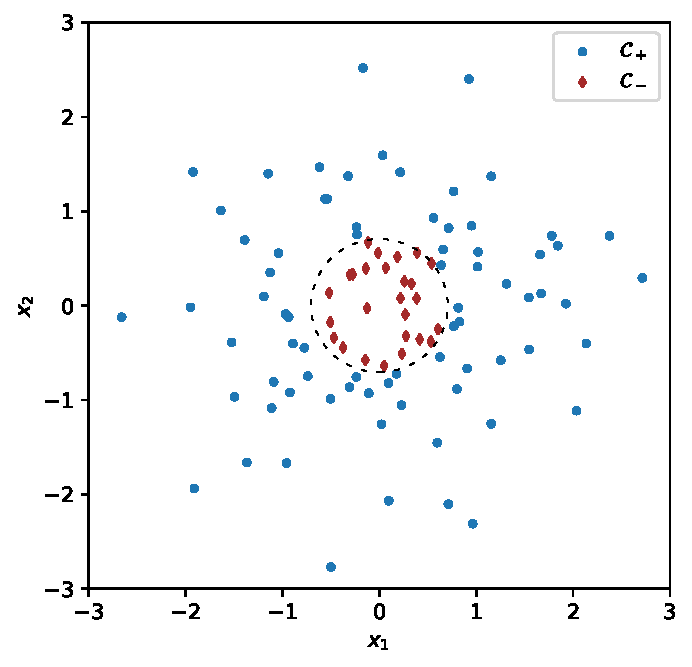
\includegraphics[width=1\linewidth]{figures/fs_subset_not_unique.pdf}
        \caption{
                Illustration of the non-uniqueness of the Markov blanket.
                Here $\cX_1 \sim \cN\left( 0, 1 \right)$,
                $\cX_2 = \cX_1^2$,
                and $\cY$ is $\cC_+$ if $\abs{\cX_1} \geq \frac{1}{2}$,
                $\cC_-$ otherwise.
                Both $\cX_1$ and $\cX_2$ alone are enough to predict $\cY$.
        }
        \label{fig:fs_subset_not_unique}
\end{wrapfigure}
Markov blanker~\cite{markov_blanket}.
We define the set of null features $\cH_0 \subseteq \fset$ as follows:
$j \in \cH_0$ if and only if $\cY \independent \cX_j \mid \cX_{-j}$
(where $\cX_{-j}$ denotes that all column entries are kept except the $j$th).
The goal is thus to find a procedure selection a subset of features
$\hat{\cS} \subseteq \fset$.

In practice, one would observe several independent realizations of
$\left( \cX,\, \cY \right)$ and would aggregate them into a feature matrix
$X \in \R^{n \times p}$ of $n$ samples and $p$ features, and a target vector $\yy \in \R^n$ respectively.
The independence of the observations is a credible assumption in many real life settings

\subsection{Motivation}\label{subsec:fs_motivation}

Feature selection may be used in a multitude of contexts
\begin{enumerate}
        \item Making the model more interpretable.
                It gives insights on the most relevant features to explain the observed target.
        \item Facilitating data visualization.
                As only a small subset of the features is selected,
                projecting it to a low (2 or 3) dimensional space is easier.
        \item Reducing the training time.
                Many machine learning algorithm have a super-linear time complexity in the number of features.as less
        \item Improving the generalization of machine learning models.
                Irrelevant features may only be noise and fitting a model against them at train time
                is prone to over-fitting noise.
\end{enumerate}


\subsection{Techniques}\label{subsec:fst}

A lot of different paradigms and techniques to perform feature selection exist~\cite{intro_fs}.

\subsubsection{Lasso}\label{subsubsec:lasso}

First introduced by Tibshirani~\cite{lasso} in 1996,
the Lasso has become increasingly popular.
It is basically a linear regression whose weights are penalized by their $\ell_1$ norm,
multiplied by some factor $\lambda > 0$.
%
\begin{equation}\label{eq:lasso}
        \hat{\bbeta}(\lambda) =
        \underset{\bb}{\argmin}\;
                \frac{1}{2}\norm{\yy - X\bb}_2^2 + \lambda\norm{\bb}_1
\end{equation}
%
The $\ell_1$ penalty tends to make the weights $\hat{\bbeta}(\lambda)$ sparse as $\lambda$ increases.
Actually, for any feature $j$,
there is a $\lambda_{\min}$ such that for all $\lambda \geq \lambda_{\min}$,
$\hat{\bbeta}_j(\lambda) = 0$.
That wouldn't be the case with an $\ell_2$ penalty,
for which the coefficients tend to $0$ without reaching that value.
This property makes the Lasso particularly suited for feature selection;
just keep the features whose weight is non-zero.
However, the choice of $\lambda$ seems to be arbitrary,
especially as it's not possible to know beforehand how many features will be selected.
The behavior of the path $\lambda \mapsto \hat{\bbeta}(\lambda)$ has been extensively studied,
and the algorithm LARS~\cite{lars} was developed to efficiently compute it
(which is possible because it is piecewise linear).
It allows to compute $\hat{\bbeta}$ for all relevant value of $\lambda$ at a marginal cost.
In practice, the $\lambda$ giving the highest score on a \emph{train} dataset is picked.


\subsubsection{Odd-Ratios}
Odd-Ratios~\cite{Mladenic1999FeatureSF}


None of the selection criterion presented above offer any guarantees regarding
the inclusion of the selected features to $\cS$.


\section{False discovery rate control}\label{sec:fdrc}
%
\subsection{Definitions}\label{subsec:fdr_def}
%
When performing feature selection one is usually interested in two quantities,
namely the \emph{false discovery rate} (FDR) and the \emph{power}.
Intuitively, the former (resp.\ the latter) assesses the expected proportion of false discoveries
(resp.\ true discoveries) of a selection procedure.
Suppose the conditional probability distribution of $\yy$ depends only on a subset
$\cS \subset \left\{ 1, \dots, p \right\}$.

We define the false discovery proportion, the false discovery rate, and the power as follows
\begin{equation}\label{eq:fdr_def}
        \fdp = \frac
                {\big\lvert\big\{ j \mid j \in \hat{\cS} \setminus \cS \big\}\big\rvert}
                {\lvert\hat{\cS}\rvert}
        \text{,}\quad
        \fdr = \Eb{\fdp}
        \text{,}\quad
        \power = \E{
                \frac
                {\big\lvert\big\{ j \mid j \in \hat{\cS} \cap \cS \big\}\big\rvert}
                {\lvert\hat{\cS}\rvert}
        }
\end{equation}

Even though it is beyond hope to retrieve the whole set $\mathcal{S}$ with no error,
a multitude of techniques attempt to find as many relevant features as possible
(that is, maximizing the power)
while maintaining the false discovery rate under a given threshold.
Controlling the FDR is particularly
In the last two decades
It is now possible to measure the expression of several dozens of thousands of genes for a given individual.

\subsection{BHq}\label{subsec:bhq}

For each feature $j \in \fset$, let $\cH_j$ be the null hypothesis ($j$ does not belong to $cS$),
and $\pvalue_j$ the corresponding $p$-value.
Let $\fdrtarget \in [0, 1]$ be some FDR target.
We note $(\pvalue_{(j)})_j$ the sequence of $p$-values in increasing order;
$\pvalue_{(1)} \leq \dots \leq \pvalue_{(p)}$.
Let $m_0$ be the number of true null hypotheses.

\subsubsection{Benjamini–Hochberg}\label{subsubsec:bh}

The Benjamini–Hochberg (BH) procedure was introduced by~\cite{bh} and allows to control the FDR under some
assumptions.
It consists in sorting the $p$-values $\pvalue_{(1)} \leq \dots \pvalue_{(p)}$,
and finding the largest $k \in \N$ such that $\pvalue_{(k)} \leq \frac{k \cdot \fdrtarget}{p}$.
Then, all the hypotheses $\cH_{(j)}$ such that $j \in \left\{ 1, \dots, k \right\}$ are rejected,
i.e.\ the feature is selected.
It guarantees that $\fdr \leq \frac{m_0}{p}\fdrtarget$ under the assumption that the $p$-values were computed
independently.

\subsubsection{Benjamini–Yekutieli}\label{subsubsec:by}

Similarly, the Benjamini–Yekutieli procedure~\cite{by} controls the FDR and does not need the independence assumption,
at the cost of a more conservative selection.
It follows the same scheme:
ordering the $p$-values,
finding the largest $k \in \N$ such that $\pvalue_{(k)} \leq \frac{k}{p \cdot c(p)}\fdrtarget$,
and rejecting $\cH_{(j)}$ if $j \leq k$.
Note the additional factor $c(p) \geq 1$, defined in~\ref{eq:by_factor}.
\begin{equation}\label{eq:by_factor}
        c(p) = \sum_{j = 1}^p \frac{1}{j}
        ,\qquad
        \fdr \leq \frac{m_0}{p}\fdrtarget
\end{equation}


Both procedures are illustrated in figure~\ref{fig:bhy}.
\begin{figure}[h]
        \centering
        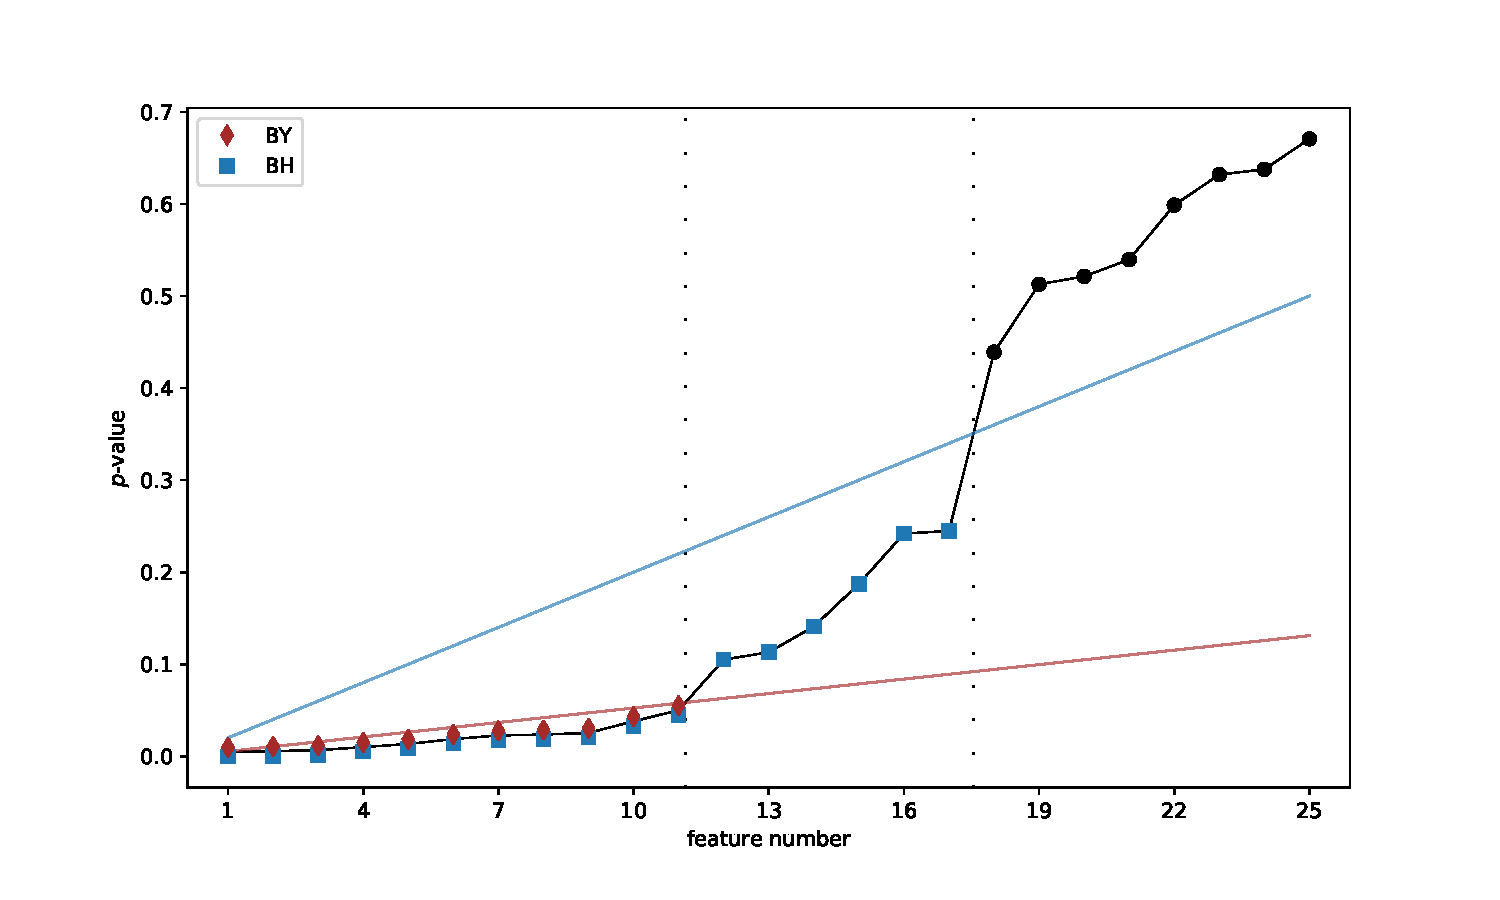
\includegraphics[width=1.\textwidth]{figures/bhy.pdf}
        \caption{
                Illustration of the BH and the BY procedures.
                They are geometrically equivalent to drawing a line of slope $\beta$ going through the origin,
                identifying the last $p$-value under the line, and keeping the features on the left.
                For BH, $\beta = \frac{\fdrtarget}{p}$ (in blue),
                while for BY, $\beta = \frac{\fdrtarget}{p \cdot c(p)}$ (in cyan).
                In this toy example, $\fdrtarget = 0.5$, and it shows that BY is way more conservative than BH.
        }
        \label{fig:bhy}
\end{figure}

Both procedures require $p$-values to be computed, which is not always feasible, especially when $p > n$.
Both the BH and the BY procedures have stronger guarantees than desired.
For a desired FDR level $\fdrtarget$,

% \cite{statistical_inference_genome}\cite{resampled_fdr_control}\cite{unified_fdr_control}

\FloatBarrier
\section{FDR control with knockoffs}\label{sec:knockoffs}

In 2015 Barber-Candès introduce the knockoffs framework and extend it later in 2018 to more general settings
(allowing in particular to perform feature selection in the high dimension context).
The goal is to control the false discovery rate as defined in~\ref{eq:fdr_def}, while maintaining a reasonable power.
More formally, let $X \in \R^{n \times p}$ be a a feature matrix and $\yy \in \R^n$ the associated target vector.
Suppose $\yy$ depends only on the subset of features $\cS \subseteq \fset$.
Given some $\fdr$ target $\fdrtarget \in [0, 1]$, we wish to find a procedure such as, in average,
the false discovery proportion is smaller that $\fdrtarget$, i.e. $\fdr \leq q$.
To do so, the key idea is to construct for each original feature $X_j$, $j \in \fset$,
a knockoff (namely, fake) feature $\tilde{X}_j$ which is known to be out of the model.
Original features are then selected only if they prove to be more significant than their knockoff counterparts.

Note $\Sigma = X^\top X$.

To compare a feature and its knockoff several quantities will be computed by interchanging them.
For this reason, we define in~\ref{def:swap} the $\swap$ operator.
\begin{definition}\label{def:swap}
        \text{($\swap$ operator)}
        We define the $\swap$ operator on the concatenated matrix $\big[ X, \tX \big]$ as follows.
        For a given subset of indices $S \subseteq \left\{ 1, \dots, p \right\}$,
        $\big[ X, \tX \big]_{\swap(S)}$ is the transformed matrix where columns $X_j$ and $\tX_j$ were swapped for all
        $j \in S$.
\end{definition}

In the following sections, we are going to detail principal aspects of the construction of the knockoff features,
the computation of statistics for both original and knockoff features,
and the feature selection based on those statistics.
%
\subsection{Knockoffs construction}\label{subsec:kc}

In 2015, Barber-Candès introduced first the \textit{fixed}-X knockoffs variable selection procedure.
It could only perform adequately when $n \geq 2p$ and be partially extended to the cases $n \geq p$.
Despite the restriction of \textit{fixed}-X knockoffs, that method is still appealing as the construction of the
knockoff variables is straightforward.
In 2018, they proposed an extension of the framework called \textit{model}-X knockoffs

In this section, let $(\cX, \cY)$ be a pair of random variables,
$\cX$ being a $p$-dimensional feature,
and $\cY$ the associated target in $\R$.
We suppose that the feature matrix and the target vector $(X,\, \yy)$ are sampled from $(\cX,\, \cY)$.
We wish to build knockoff features $\tX \in \R^{n \times p}$, and to do so we are going to sample from a
random variable $\tcX$ built such that $\big[ \cX; \tcX \big]$ follows some properties.

\begin{definition}
\text{(model-$X$ knockoffs)}
Given random vector $\cX \in \R^p$ of features,
a random vector $\tcX \in \R^p$ is said to be model-$X$ knockoffs with respect to $\cY$
if it satisfies the two following properties:
\begin{enumerate}[label=\textbf{S.\arabic*},ref=S.\arabic*]
        \item \label{itm:cond_swap} For any $S \subseteq \fset$,
                $\big[ \cX, \tcX \big]_{\swap(S)} \distreq \big[ \cX, \tcX \big]$
        \item \label{itm:cond_indep} $\tcX \independent \cY \mid \cX$
\end{enumerate}
\end{definition}
The independence condition~\ref{itm:cond_indep} is trivially satisfied if $\tX$ is built without exploiting $\yy$.
However, constructing knockoffs meeting the first distribution equality is practically infeasible in general.
In the particular case where $X$ is gaussian, the exact distribution of $\tX$ can be derived.
\begin{proposition}
        Suppose $\cX \sim \cN(\bmu, \Sigma)$.
        If $\tcX$ is such that
        \begin{equation*}
                \big[ \cX; \tcX \big] \sim \cN\bigg(\begin{bmatrix} \bmu\\ \bmu \end{bmatrix}, \Omega\bigg)
                ,\quad\text{where}\quad
                \Omega = \begin{bmatrix}
                         \Sigma & \Sigma - \diag \bs\\
                         \Sigma - \diag \bs & \Sigma
                \end{bmatrix}
                \text{for some }
                \bs \in \R^p
        \end{equation*}
        then $\big[\cX, \tcX \big]$ satisfies the $\swap$ property~\ref{itm:cond_swap},
        provided that $\Omega$ is positive semidefinite,
        which is equivalent to $\0_{p \times p} \preceq \diag \bs \preceq 2\Sigma$.
\end{proposition}\label{prop:gaussian_knockoffs}
The proposition~\ref{prop:gaussian_knockoffs} gives a way to construct the knockoff features in the case were
$\cX$ is gaussian.
Indeed, as $\big[ \cX; \tcX \big]$ is multivariate normal, we may compute the exact distribution of
$\tcX \mid \cX$ with classical formulas~\cite{conditional_normal} as shown in~\ref{eq:conditional_gaussian_knockoffs}.
\begin{equation}\label{eq:conditional_gaussian_knockoffs}
        \tcX \mid \cX \sim \cN\left( \bmu, \Upsilon \right)
        ,\qquad\text{where}\quad
        \begin{cases*}
                \bmu = \cX - \cX\Sigma^{-1}\diag(\bs)\\
                \Upsilon = \diag(\bs)\left( 2\mI - \Sigma^{-1}\diag(\bs) \right)
        \end{cases*}
\end{equation}
To put this into practice, one would compute the empirical mean
$\hat{\bmu} \in \R^p$ and covariance $\hat{\Sigma} \in \R^{p \times p}$ of $\cX$
using the observed feature matrix $X$.
Then, each row is sampled according to a gaussian distribution whose parameters are described
in~\ref{eq:conditional_gaussian_knockoffs}.
Note in particular that the construction process is random;
if it is repeated, it may very well return different knockoffs, and thus different
selected features.
Because of this instability, several attempts~\cite{improve_stability_knockoffs} to fix it by
aggregating several knockoff samples.

The gaussian hypothesis is obviously rarely verified in practice but yields acceptable results even when
$\cX$ is far from gaussian.
It partly comes from the fact that, rather than constructing $\tcX$ to respect~\ref{itm:cond_swap},
a weaker condition would be to enforce $\big[ \cX, \tcX \big]$ and $\big[ \cX, \tcX \big]_{\swap(S)}$ to have the
same mean and covariance.
It turns out to be the case if $\tcX \mid \cX$ is constructed as in~\ref{eq:conditional_gaussian_knockoffs}.
In the remaining of this master thesis, we will restrain ourselves to the gaussian hypothesis.

Constructing the knockoffs feature matrix $\tmX \in \R^{n \times p}$.
It must satisfy two conditions, namely:
\begin{align*}
        &{\tmX}^\top\tmX = \mSigma,
        \\
        &\mX^\top\tmX = \mSigma - \diag\{\bs\}
        \text{ where } \bs \text{ is a non negative vector.}
\end{align*}
It ensures that $\tilde{\mX}$ has the same covariance as the original matrix $\mX$
and that the correlation between distinct original and knockoff variables is the same as the correlation between the
two originals.
Barber-Candes detail several approaches to construct this knockoff matrix $\tilde{\mX}$.
It is easiest in the case where $n \geq 2p$.

\subsection{Statistics computation}\label{subsec:ksc}

Given the original feature matrix and the sampled knockoffs $X,\, \tX \in \R^{n \times p}$,
statistics $w_j$ for all $j \in \fset$ are computed.
These statistics must satisfy the \emph{flip-sign} technical condition~\ref{def:flip_sign} for the method to work,
but a wide variety of choices is possible as will be shown.
\begin{definition}\label{def:flip_sign}
        \text{(flip-sign property)}
        A statistics function $\omega \colon \R^{n \times 2p} \times \R^n \to \R^p$
        is said to follow the flip-sign property if for any $S \subseteq \fset$ and any $j \in \fset$,
        \begin{equation*}
                \omega_j\big( \big[ X, \tX \big]_{\swap(S)},\, \yy \big) = \begin{cases*}
                        -\omega_j\big( \big[ X, \tX \big]_{\swap(S)},\, \yy \big) &\quad\text{if $j \in S$.}\\
                        \omega_j\big( \big[ X, \tX \big]_{\swap(S)},\, \yy \big) &\quad\text{otherwise.}
                \end{cases*}
        \end{equation*}
\end{definition}

\subsection{Statistics aggregation}\label{subsec:ksa}

Constructing statistics satisfying the \emph{flip-sign} property~\ref{def:flip_sign} is actually straightforward
as a simple scheme leads to such statistics.
The idea is to build statistics for each original and each knockoff feature, and then aggregate them.
First construct statistics $[ \zz ; \tilde{\zz} ] = \zeta\big( \big[ X, \tX \big],\, \yy \big)$
with some function $\zeta \colon \R^{n \times 2p} \times \R^n \to \R^{2p}$ satisfying
\begin{equation}\label{eq:swap_cond}
        [ \zz ; \tilde{\zz} ]_{\swap(S)} = \zeta\big( \big[ X, \tX \big]_{\swap(S)},\, \yy \big)
        ,\quad
        \forall S \subseteq \fset
\end{equation}
The statistics $z_j$ (resp. $\tilde{z}_j$) indicates how significant the original (resp.\ knockoff) feature $j$ is.

Then aggregate for each $j \in \fset$ the statistics of the original feature $z_j$ and the one of the corresponding
knockoff $\tilde{z}_j$ with an antisymmetric function $a_j \colon \R\times\R \to \R$,
that is, set $w_j = a_j(z_j, \tilde{z}_j)$.
Basically any antisymmetric function could work, but some choices lead to better statistics.
As for the function $\zeta$, it only needs to satisfy the \emph{swap} property~\ref{eq:swap_cond}.
This condition may seem restrictive but a large number of choices are actually valid.

Computing antisymmetric statistics $\ww \in \R^p$ where $\forall j = 1, \dots, p$, $w_j$
indicates how more important an original feature $j$ is compared to its associated knockoff.
Several mappings are possible, for example:
\begin{itemize}
        \item $w_j = z_j - \tilde{z}_j$ (experimentally gives highest power)
        \item $w_j = \max(z_j, \tilde{z}_j) \times \sign(z_j - \tilde{z}_j)$ (first proposed in 2015)
        \item $w_j = \log\frac{z_j}{\tilde{z}_j}$
\end{itemize}
Barber-Candès suggest the following one after empirical observations.
Let $\hat{\bbeta}(\lambda) = \underset{\bb}{\operatorname{argmin}}
\{\frac{1}{2}\norm{\yy - \mX\bb}_2^2 + \lambda\norm{\bb}_1\}$.
Define then $z_j = \sup\{\lambda \mid \mathbf{\hat{\beta}}_j(\lambda) \neq 0\}$.
Intuitively, it is the first $\lambda$ such that the feature enters in the model.
There are other ways to compute the $z_j$ statistics.
It would for example be possible to train a regressor and take the absolute values of its coefficients.

\subsection{Features selection}\label{subsec:kfs}

The selection itself requires the computation of a data-dependent threshold $\tau$
conditioned by the target FDR $\fdrtarget$, as defined in~\ref{eq:knock_thres} and~\ref{eq:knockp_thres}.
Finally, features $j$ whose statistics $w_j$ are above the threshold are selected;
$\hat{\cS} = \left\{ j \mid w_j \geq \tau \right\}$.
Depending on how selective we want the procedure to be, the threshold $\tau$ can be adapted,
and leads to different guarantees regarding the control of the FDR\@.
Let's first define a modified version of the FDR\@.
\begin{definition}\label{def:mfdr}
        Given an estimate $\hat{\cS}$ of $\cS$ and a desired target false discovery rate $q \in [0, 1]$,
        we define the modified $\fdr$ as follows:
        \begin{equation*}
                \mfdr = \E{
                \frac
                {\abs{\left\{ j \mid j \in \hat{\cS} \setminus \cS \right\}}}
                {\lvert\hat{\cS}\rvert + 1 / q}
                }
        \end{equation*}
\end{definition}
As $q \leq 1$, $\mfdr$ as defined in~\ref{def:mfdr} is always smaller than the actual $\fdr$.
But if the target threshold $q$ is not too low, and if many features are selected by the procedure,
the modified version of the FDR is close enough to the true value.
Controlling it is then relevant.
\begin{definition}
        (knockoff and knockoff+ thresholds)
        \begin{align}
                \tau &=
                        \min\left\{
                                t > 0 \mid \frac{\abs{j \mid w_j \leq -t}}{\abs{j \mid w_j \geq t}} \leq q
                        \right\}\label{eq:knock_thres}\\
                \tau^+ &=
                        \min\left\{
                                t > 0 \mid \frac{1 + \abs{j \mid w_j \leq -t}}{\abs{j \mid w_j \geq t}} \leq q
                        \right\}\label{eq:knockp_thres}
        \end{align}
\end{definition}

\begin{theorem}
        Construct $\hat{\cS} = \left\{ j \mid w_j \geq \tau \right\}$
        and $\hat{\cS}^+ = \left\{ j \mid w_j \geq \tau^+ \right\}$.
        Then,
        \begin{equation}
                \mfdr\left[ \hat{\cS} \right] \leq q
                ,\qquad
                \fdr\left[ \hat{\cS}^+ \right] \leq q
        \end{equation}
\end{theorem}
%
\subsection{Bottlenecks}\label{subsec:kb}

Despite the nice theoretical guarantees on the $\fdr$ control that the knockoff procedure proposes,
two bottlenecks hurt its performances in the high dimensional setting.

\subsubsection{SDP}\label{subsubsec:bot_sdp}

Knockoff features are sampled according to the distribution~\ref{eq:conditional_gaussian_knockoffs},
and the results hold for any $\bs \in \R^p$ such that the covariance matrix is semidefinite positive.

\begin{proposition}
        Let $\Omega = \begin{bmatrix}
                             \Sigma & \Sigma - \diag \bs\\
                             \Sigma - \diag \bs & \Sigma
        \end{bmatrix}$.
        Then $\Omega \succeq \0_{p \times p}$ if and only if $2\Sigma \succeq \diag \bs \succeq \0$.
\end{proposition}

\begin{proof}
        Note $D = \diag\bs$.
        By computing the Schur complement~\cite{schur_complement}
        $\Omega_{/\Sigma} = 2D - D\Sigma^{-1}D$,
        $\Omega \succeq \0$ is equivalent to $\Omega_{/\Sigma} \succeq \0$.
        Define $M$ and its Schur complements as follows
        \begin{equation*}
                M = \begin{bmatrix}
                        2D & D\\
                        D & \Sigma
                \end{bmatrix}
                ,\qquad\qquad
                \begin{cases*}
                        M_{/2D} = \Sigma - \frac{1}{2}D\\
                        M_{/\Sigma} = 2D - D\Sigma^{-1}D
                \end{cases*}
        \end{equation*}
        Finally, $\Omega_{/\Sigma} = M_{/\Sigma}$ is p.s.d.\ if and only if both $\Sigma - \frac{1}{2}D$ and $D$ are p.s.d.
\end{proof}

\subsubsection{Statistics computation}\label{subsubsec:bot_stats}

and could take advantage of sparse naive Bayes to run faster.
\bigbreak
These two bottlenecks make the .
The following chapters tackle these two issues by proposing fast statistics computation.
From now, only binary classification problems will be considered, where the label $y$ takes values
in $\left\{ \cC^+,\, \cC^- \right\}$.

\subsection{Python implementation}\label{subsec:python_implementation}

Barber-Candès (along with other coauthor) provided a R implementation
of the knockoff framework\footnote{
        The package page can be found at this address \url{https://cran.r-project.org/web/packages/knockoff/index.html}.
}.
To the best of our knowledge, no unified Python implementation
Scikit-Learn~\cite{sklearn}
